\documentclass[11pt]{article}
\usepackage[utf8]{inputenc}
\usepackage[T1]{fontenc}
\usepackage{amsmath}
\usepackage{amsfonts}
\usepackage{amssymb}
\usepackage[version=4]{mhchem}
\usepackage{stmaryrd}
\usepackage{multirow}
\usepackage{graphicx}
\usepackage[export]{adjustbox}
\graphicspath{ {./images/} }

\begin{document}
Visual Works of Art and Historical Performance Data

Within IP, art tends to provide superior long-term pricing data for analysis of historical returns. Visual works of art include paintings and have a rich history of prices and returns, but they do not represent a major component of institutional portfolios. Further, returns from previous centuries are probably not reflective of returns related to modern market conditions. It should be noted that art is a major component of some high-net-worth investor portfolios.

There is a wide range of studies regarding the returns to art, typically differentiated by style or geography, as reflected in the next exhibit, Estimated Returns to Art from Various Studies. The median real return to holding art over extended periods of time is $2.2 \%$ (methods used to estimate returns do not vary substantially in outcomes). However, most studies of the returns to art investment consider only hammer prices, which are final auction prices that do not include commissions to the auction house. Commissions that may be charged to both the buyer and the seller amount to as much as $15 \%$. If we assume that the typical round-turn transaction cost for a sale is $25 \%$, then it would be expected to take 10 years of price appreciation to cover the transaction costs associated with a piece of art.

Estimated Returns to Art from Various Studies

\begin{center}
\begin{tabular}{|c|c|c|c|c|c|}
\hline
Author & Sample & Period & Method & Nominal Return & Real Return \\
\hline
\multirow[t]{2}{*}{Anderson (1974)} & Paintings in general & $1780-1960$ & Hedonic & $3.3 \%$ & $2.6 \%$ \\
\hline
 & Paintings in general & $1780-1970$ & Repeat sales & $3.7 \%$ & $3.0 \%$ \\
\hline
Stein (1977) & Paintings in general & 1946-1968 & Assumes random sampling & $10.5 \%$ &  \\
\hline
Baumol (1986) & Paintings in general & 1652-1961 & Repeat sales &  & $0.6 \%$ \\
\hline
\multirow[t]{2}{*}{Frey and Pommenihne (1989)} & Paintings in general & $1635-1949$ & Repeat sales &  & $1.4 \%$ \\
\hline
 &  & 1950-1987 & Repeat sales &  & $1.7 \%$ \\
\hline
Buelens and Ginsburgh (1993) & Paintings in general & $1700-1961$ & Hedonic &  & $0.9 \%$ \\
\hline
Pesando (1993) & Modern prints & 1977-1991 & Repeat sales &  & $1.5 \%$ \\
\hline
Goetzmann (1993) & Paintings in general & 1716-1986 & Repeat sales & $3.2 \%$ & $2.0 \%$ \\
\hline
\multirow[t]{2}{*}{Barre et al. (1996)} & Great impressionist & 1962-1991 & Hedonic & $12.0 \%$ & $5.0 \%^{\mathrm{a}}$ \\
\hline
 & Other impressionist & 1962-1991 & Hedonic & $8.0 \%$ & $1.0 \% \mathrm{a}$ \\
\hline
\multirow[t]{2}{*}{Chanel et al. (1996)} & Paintings in general & 1855-1969 & Hedonic &  & $4.9 \%$ \\
\hline
 & Paintings in general & 1855-1969 & Repeat sales &  & $5.0 \%$ \\
\hline
Goetzmann (1996) & Paintings in general & 1907-1977 & Repeat sales &  & $5.0 \%$ \\
\hline
Pesando and Shum (1996) & Picasso prints & 1977-1993 & Repeat sales & $12.0 \%$ & $1.4 \%$ \\
\hline
Czujack (1997) & Picasso printings & 1966-1994 & Hedonic &  & $8.3 \%$ \\
\hline
Mei and Moses (2001) & American, impressionist, and old master & $1875-2000$ & Repeat sales &  & $4.9 \%$ \\
\hline
Graeser (1993) & Antique furniture & $1967-1986$ & Neither ${ }^{b}$ & $7.0 \%$ & $2.2 \%$ \\
\hline
Ross and Zondervan (1989) & Stradivarius violins & 1803-1986 & Hedonic &  & $2.2 \%$ \\
\hline
\end{tabular}
\end{center}

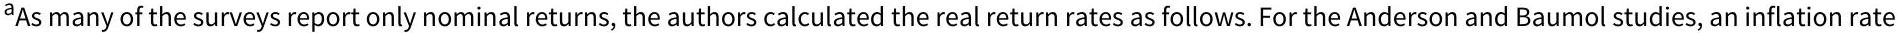
\includegraphics[max width=\textwidth, center]{2024_04_11_14fb13b1a1f6b829d6b6g-2}\\
of $0.7 \%$ a year was used. This number is based on Baumol's estimate of inflation during the 300 -year period of his study using the Phelps-Brown and Hopkins price index. Goetzmann's estimate of inflation during the period of his study (also based on Phelps-Brown and Hopkins) is 1.2\%. French price inflation between 1962 and 1992 according to OECD statistics was 7\%.

${ }^{\mathrm{b}}$ Assumes random sampling within a portfolio of fixed furniture types.

Source: Ashenfelter and Graddy (2003).

Spaenjers (2010) considers data on more than 1 million art transactions across 13 countries from the 1960s onward, accounting for both geographical and currency effects. The results are consistent with the preceding: Annualized real returns to a diversified basket of art have been in the neighborhood of $2 \%$ and do not vary significantly across geographies or markets. In addition, the volatility of art indices has a median of $17 \%$ per year. This combination of risk and return compares unfavorably to historical experience in equity markets. In other words, the Sharpe ratio is relatively unattractive.

Forsyth (2012) suggests that high-net-worth investors invest in art as a hedge against inflation or confiscation of wealth by governments. For those with a net worth above $\$ 100$ million, he suggests, an important goal is to maintain rather than grow wealth. Artworks can protect against monetary debasement, confiscation, and social unrest. Forsyth quotes Richard Morais: "Any private banker will tell you that, as soon as a centimillionaire ... makes their fortune, the first thing they do is figure out how they can ferret away large chunks of that wealth to countries that guarantee political and personal freedoms, have sound legal systems, a favorable tax environment, good security and good schools for their kids." A substantial portion of this newfound wealth may be invested in real estate in cities such as New York or London, and in art, which can be easily shipped to the residences in these safe, global cities.

Another explanation of low financial returns to art is that the investment in art provides a total return that is a combination of the financial return to art (price appreciation) and the aesthetic benefit to being the owner of the art. The aesthetic benefit is the nonfinancial benefit to owning art and includes the joy of viewing and otherwise controlling the art. To the extent that competition drives the total return to similar risk-adjusted levels, there is a trade-off between the financial return and the aesthetic benefit. In artwork overall, and perhaps in some artwork in particular, prices are driven higher (and expected financial returns are driven lower) in anticipation of the nonfinancial benefits from ownership.

The historical evidence of modest real returns and nontrivial risk indicates disappointing risk-adjusted financial returns. Economic reasoning indicates that one explanation is that art offers part of its return in the form of aesthetic benefits. Although art can be attractive as a wealth-preservation technique for high-net-worth investors, there is little basis for viewing it as an attractive asset class for traditional financial institutional portfolios.


\end{document}